\section{BioMérieux Solution}

\begin{figure}[h]
    \centering
    
\includegraphics[scale=0.5]{img/bmx.png}
    \caption{Logo de bioMérieux}
\end{figure}

BioMérieux est une entreprise spécialisée dans le diagnostic in vitro et dans la microbiologie.
Cette entreprise concoit et fabrique des instruments permettant de diagnostiquer des maladies et de faire des analyses microbiologiques.
BioMérieux dispose d'un showroom permettant de montrer leur produits à leurs futurs clients.

\subsection{Situation initial}

Dans ce Showroom, un ensemble de dispositifs interactifs sont mis en place pour presenter les produits et l'entreprise.
Parmis ces équipements, on retrouve l'espace solution.
Cet espace présente un exemplaire physique des principales machines concus par bioMérieux.
Un projecteur permet alors d'afficher une image sur une vitre opacifiante.
L'image projetée est l'écran d'un Mac Mini disposé dans la salle technique du Showroom;
On utilise un lidar\footnote{Le lidar est un laser rotatif permettant, par balayage, de detecter la position d'un element dans l'espace} pour reperer l'emplacement du doigt sur la vitre et ainsi controler l'ordinateur.

L'application présente avant ma mission etait développée en C++ avec OpenFrameworks.
Cette application présente un arbre de composents graphiques chacun affichant un élément de l'interface.
Ce système, bien que fonctionnel, est assez peux flexible au regard des nouvelles fonctionnalités demandés par bioMérieux.

En effet, bioMérieux à recemment changé son logo et sa charte graphique pour un aspect plus épuré et flat-design\footnote{Le flat-design est un courant de design moderne qui possède une approche minimaliste de l'interface en se basant sur des aplats de couleurs unis et des effets d'ombres}.
Pour reflèter ce changement dans leur showroom, l'entreprise a demandé un redesign de l'application.
De plus, pour pouvoir gèrer par eux même les produits presents dans l'application, bioMérieux a demandé la mise en place d'un backoffice qui permettra d'éditer le contenu de l'application sans faire appel à LTBL.

\begin{figure}[h]
    \centering
    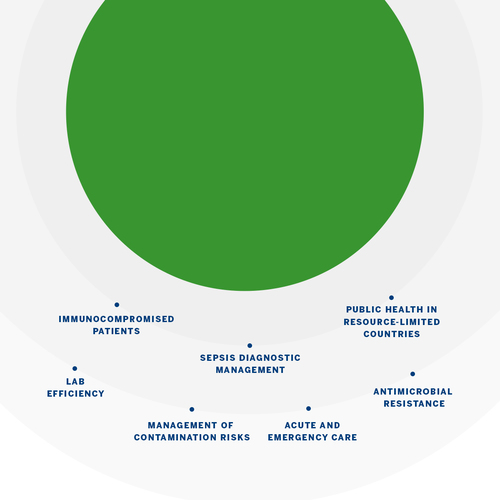
\includegraphics[scale=0.195]{img/resized-bmx-1-new.jpg}
    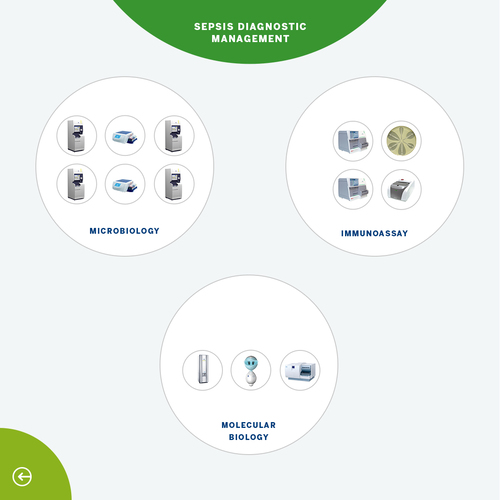
\includegraphics[scale=0.195]{img/resized-bmx-2-new.jpg}
    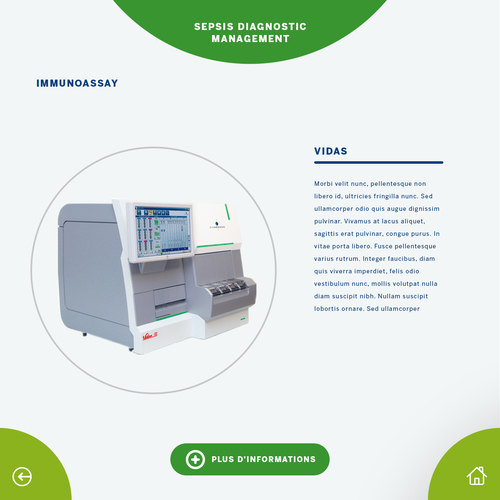
\includegraphics[scale=0.195]{img/resized-bmx-3-new.jpg}
    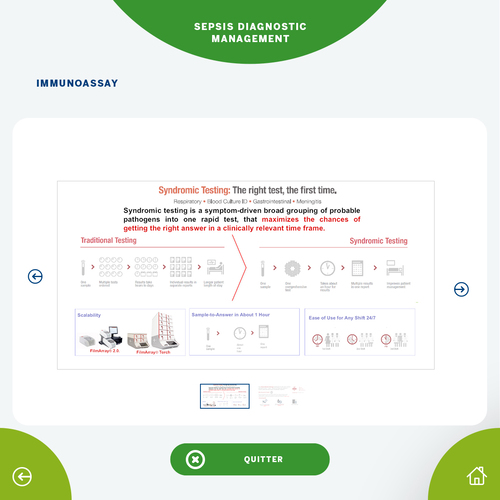
\includegraphics[scale=0.195]{img/resized-bmx-4-new.jpg}
    \caption{Design renouvelé de l'application Biomérieux}
\end{figure}

Enfin, dans une optique de recherche et développement d'une soltion universelle de backoffice chez LTBL il fallait aussi réfléchir à un système flexible de stockage de données.

Pour résumer, les fonctionnalités demandés sont :

\begin{itemize}
    \item La mise à jour de la charte graphique de bioMérieux
    \item La mise en place d'un backoffice pour gèrer les produits
    \item Faire en sorte que le backoffice puisse être réutilisé dans d'autres projets LTBL
\end{itemize}


\subsection{Conception de la solution}

Le code précédent etant totalement fait main, il est peu flexible et sensible aux bugs de développement.
De plus les données sont dirèctement intègrés dans le code et il serait chronophage et peu rentable de modifier cette application pour qu'elle d'adapte aux nouveaux besoins.
J'ai donc décide de reprendre l'application depuis le début et de choisir une solution technique qui me semble plus adaptée à une interface.

\subsubsection{Electron}

Pour développer l'application j'ai décidé d'utiliser Electron.

\begin{figure}[h]
    \centering
    
\includegraphics[scale=0.5]{img/electron.png}
    \caption{Logo de Electron}
\end{figure}

Electron est un framework permettant de concevoir des application natives en utilisant les technologies web.
Electron embarque le moteur de rendu et le moteur Javascript de chromium mais ajoute les fonctionalités de NodeJS permettant d'interagir avec le système hote.

L'utilisation de ce framework est interessante dans le cas de cette application car elle permet de concevoir des interfaces simplement.
